
\chapter{Proving more complex statements}


\section{Syntax Trees}

In the chapter on connectives, we analyzed the following two propositions:

\begin{enumerate}
	\item $\exists x \in \mathbb{R}: [(2x+1 = 5) \wedge (3x+3 = 5)]$
	
	\item $[\exists x \in \mathbb{R}: (2x+1 = 5)] \wedge [\exists x: (3x+3 = 5)]$
\end{enumerate}

Understanding the difference between these two statements may have been difficult for you.  Here we will introduce another way to record the logical structure of these sentences called a \textbf{syntax tree} which might be a little easier to understand (once you get the hang of it).

Statement (1) is existentially quantifying the predicate $[(2x+1 = 5) \wedge (3x+3 = 5)]$ in the variable $x$.  I will record this by having the \textbf{root node} of the syntax tree be $\exists x \in \mathbb{R}$, drawing a single vertical \textbf{branch} down from that node and then putting the syntax tree for the predicate $[(2x+1 = 5) \wedge (3x+3 = 5)]$ below it:

\begin{center}
	\begin{forest}
		[\(\exists x \in \mathbb{R}\)[Tree for ``\({(2x+1 = 5) \wedge (3x+3 = 5)}\)'']]
	\end{forest}
\end{center}

Since the predicate $[(2x+1 = 5) \wedge (3x+3 = 5)]$ is a conjunction of the two predicates $2x+1 = 5$ and $3x+3 = 5$, the tree for this predicate will have a root of $\wedge$, two branches, with $2x+1 = 5$ on the left and $3x+3 = 5$ on the right:

\begin{center}
	\begin{forest}
		[\(\exists x \in \mathbb{R}\)[\(\wedge\)[\({2x+1 = 5}\)][\({3x+3 = 5}\)]]]
	\end{forest}
\end{center}

The  final \textbf{leaves} at the bottom of this tree do not contain any logical connectives or quantifiers.  Each variable appearing in the leaves can be traced back to a single quantifier which introduces the variable.

However, the syntax tree for (2) would look like:

\begin{center}
	\begin{forest}
		[\(\wedge\)[\(\exists x \in \mathbb{R}\)[\( {2x+1 = 5}\)]][\(\exists x \in \mathbb{R}\)[\( {3x+3 = 5}\)]]]
	\end{forest}
\end{center}

Note that the ``tree'' analogy is a bit strange since it is upside down!  The root is at the top, and the leaves are at the bottom!  The reason for this strange convention is that we usually like to work from top to bottom when writing on a page in English.

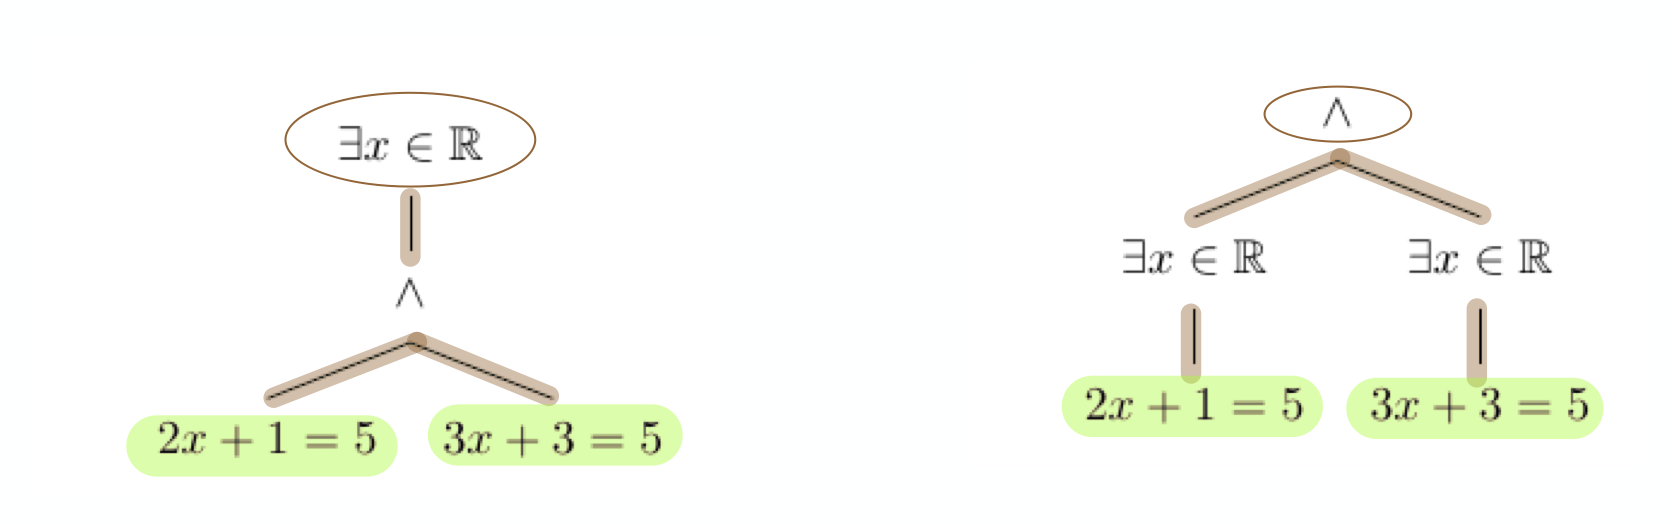
\includegraphics[scale = 0.4]{trees}

Here the root is circled, the branches are colored brown, and the leaves are colored green.

Comparing these two we see that in (1) the existential quantification of $x$ applies to both statements $2x+1 = 5$ and $3x+3  = 5$.  We would say that both instances of $x$ are within the \index{scope}\textbf{scope} of this existential quantifier.  However, in (2) the scope of the exitential quantifier on the left branch only includes the $x$ in $2x+1  = 5$, while the scope of the existential quantifier on the right branch only includes the $x$ in $3x+3 = 5$.

\begin{example}
	Assume that $P$, $Q$, and $R$ are propositions and $A$, $B$, and $C$ are predicates. The syntax tree for 
	
	\[
	\exists x :[( P \wedge A(x)) \wedge ( \forall y( B(x) \wedge C(x,y) ))]
	\]
	
	is
	
	\begin{center}
		\begin{forest}
			[\(\exists x\)[\(\wedge\)[\(\wedge\)[\(P\)][\(A(x)\)]][\(\forall y \)[\(\wedge\)[\(B(x)\)][\({C(x,y)}\)]]]]]
		\end{forest}
	\end{center}
	
	The two dimensional layout of the tree makes some features of the expression easier to parse than when we leave it as a one dimensional written expression.
\end{example}

Since the root of this tree is an existential quantifer, I will call this an ``existentially quantified proposition''.

We will categorize all sentences this way, according to their roots:

\begin{table}[h]
	\centering
	\begin{tabular}{c|l|l}
		Root & Formal Name & Informal Name 	\\ \hline
		$\wedge$ & Conjunction & ``and'' sentence\\ \hline
		$\implies$ & Implication & ``implies'' sentence\\ \hline
		$\bi$ & Biconditional & ``if and only if'' sentence\\ \hline
		$\neg$ & Negation & ``not'' sentence\\ \hline
		$\vee$ & Disjunction & ``or'' sentence\\ \hline
		$\forall$ & Universally quantified sentence & ``for all'' sentence\\ \hline
		$\exists$ & Existentially quantified sentence & ``there exists'' sentence\\ \hline
	\end{tabular}
\end{table}

\begin{xca}
	Build a syntax tree for each of the following statements.  Assume that $P$, $Q$, and $R$ are propositions and $A$, $B$, and $C$ are predicates.  Matching parenthesis can be a struggle:  this is part of the reason why trees can be a useful way of writing these expressions.  Then categorize the sentence according to its root node.
	
	\begin{enumerate}
		\item $\forall x:  (P \wedge \exists y (A(x,y) \wedge B(x)))$
		\item $P \wedge (Q \wedge \exists t (B(t,t)) )$
		\item $\forall x: ( \exists y (A(x,y)) \wedge \forall y (C(x,y)))$
	\end{enumerate}
\end{xca}


\begin{solutions}
	\begin{enumerate}
		\item $\forall x:  (P \wedge \exists y (A(x,y) \wedge B(x)))$
		
		\begin{center}
			\begin{forest}
				[\(\forall x\)[\(\wedge\)[\(P\)][\(\exists y\)[\(\wedge\)[\({A(x,y)}\)][\(B(x)\)]]]]]
			\end{forest}
			This is a universally quantified proposition.
		\end{center}
	

	
		\item $P \wedge (Q \wedge \exists t (B(t,t)) )$
		
		\begin{center}
			\begin{forest}
				[\(\wedge\)[\(P\)][\(\wedge\)[\(Q\)][\(\exists t\)[\({B(t,t)}\)]]]]
			\end{forest}
		
		This is a conjunction.
		
		\end{center}
		\item $\forall x: ( \exists y (A(x,y)) \wedge \forall y (C(x,y)))$
		
		\begin{center}
			\begin{forest}
				[\(\forall x\)[\(\wedge\)[\(\exists y\)[\({A(x,y)}\)]][\(\forall y\)[\({C(x,y)}\)]]]]
			\end{forest}
		
		This is a universally quantified proposition.
		\end{center}
		
	\end{enumerate}
\end{solutions}

\begin{xca}
	Consider the syntax tree
	
	\begin{center}
		\begin{forest}
			[$\forall x$[$\wedge$[$\exists y$[${A(x,y)}$]][$\forall y$[$\wedge$[$P$][${B(x,y)}$]]]]]
		\end{forest}
	\end{center}
	
	Indicate all variables which are in the scope of $\forall y$.  Then convert this syntax tree to a linear string with appropriate parentheses. 
	
\end{xca}

\begin{solutions}
	The only variable within the scope of $\forall y$ is the $y$ in $B(x,y)$.
	
	We can write this proposition on one line as
	
	\[
	\forall x: (  (\exists y: ( A(x,y)))  \wedge (\forall y: ( P \wedge  B(x,y)))  )
	\]
	
\end{solutions}

\section{Fitch Style Proof Outlines}

We have seen that we can make the logical structure of mathematical statements clearer by translating them into statements in first order logic.  That is to say, if we declare the meaning of sentences like $p$, $q$, $r$,  and predicates like $A(x)$,  $B(x)$,  $C(x,y)$, then we can use the logical connectives $\wedge$, $\implies$, $\bi$, $\neg$, $\vee$ and the quantifiers $\forall$ and $\exists$ to translate mathematical statements in English into more formal and precise statements using these symbols.

For example, if we let $E(x)$ be the predicate ``$x$ is even'', then we can translate the English mathematical sentence 

{ \begin{center}
		``The product of any two even numbers is even.''
		\end{center}
}

into a symbolic form where its logical structure is more apparent:

$$
\forall x \in \Z \, \forall y \in \Z \left( E(x) \wedge E(y) \implies E(x+y) \right)
$$

or as a syntax tree:

\begin{center}
\begin{forest}
	[$\forall x \in \Z$[$\forall y \in \Z$[$\implies$[$\wedge$[$E(x)$][$E(y)$]][$E(x+y)$]]]
]
\end{forest}
\end{center}

We will see how to use this logical structure to make a ``Fitch Style Proof Outline''  for the theorem.  We will generate this outline recursively, moving down the tree.  Proving theorems in mathematics requires considerable creativity, but that creativity often lives in the ``blank spaces'' of this outline, not in the structure of the outline itself.  For each of the five connectives, and two quantifiers, we will see how to both \textbf{use} (eliminate) a statement whose root node is of that form, and how to \textbf{prove} (introduce) a statement whose root node is of that form.

On the next page we provide a summary table for the elimination and introduction rules for each node.

\newpage
	


\begin{table}[h]
	\centering
	\begin{tabular}{c?p{5 cm}?p{4 cm}}
		Root Node & How to use it if it is true (Elimination)& How to prove that it is true (Introduction)	\\ \hline 
		$p \wedge q$ & You can conclude that $p$ is true and you can conclude that $q$ is true.  & \begin{fitch*}
				\textrm{Argue $p$.}\\
				\textrm{Argue $q$.}
			\end{fitch*} \\ \hline
		$p \implies q$ & If you also know $p$ is true, then you know $q$ is true. & \begin{fitch*}
			\textrm{Assume $p$ is true.} \\
			\fa \textrm{Argue that $q$ is true.}
		\end{fitch*}\\ \hline
		$p \bi q$ & If you know the truth value of one, then the truth value of the other is identical. &  
		\begin{fitch*}
			\textrm{Assume $p$ is true.} \\
			\fa \textrm{Argue that $q$ is true.}\\
			\textrm{Assume $q$ is true.} \\
			\fa \textrm{Argue that $p$ is true.}
		\end{fitch*}
		\\ \hline
		$\neg p$ & If you also know $p$, then you can conclude $F$ (hence you can conclude anything by the principle of explosion) &  
		\begin{fitch*}
			\textrm{Assume $p$}\\
			\fa \textrm{Argue $F$}
		\end{fitch*}
		\\ \hline
		$p \vee q$ & If you are trying to argue $r$ is true, then you must split your argument into cases.
		\begin{fitch*}
			\textrm{Case 1: Assume $p$ is true.}\\
			\fa \textrm{Argue $r$ is true.}\\
			\textrm{Case 2:  Assume $q$ is true.}\\
			\fa \textrm{Argue $r$ is true.}
		\end{fitch*}
		&  Argue $p$ is true.
		
		\medskip
		
		OR
		
		\medskip
		
		Argue $q$ is true.

		\\ \hline
		$\forall x: A(x)$ & If $x_1$ is any element of the universe of discourse, you know that $A(x_1)$ is true. &  Let $x_1$ be an arbitrary element of the universe of discourse, and argue that $A(x_1)$ is true. \\ \hline
		$\exists x: B(x)$ & You know that there is at least one (and potentially only one) element of your universe of discourse which makes $B$ true.  Pick one and call it $x_1$.  You may freely use that $B(x_1)$ is true in your argument. &  You need to come up with a candidate $x_1$ for which you think $B(x_1)$ is true.  Often, this will be a formula in terms of previously declared variables.  Then argue that $B(x_1)$ really is true.
	\end{tabular}
\end{table}

\newpage


Now lets see how to make a proof outline for 

$$
\forall x \in \Z \, \forall y \in \Z \left( E(x) \wedge E(y) \implies E(x+y) \right)
$$

\begin{center}
	\begin{forest}
		[$\forall x \in \Z$[$\forall y \in \Z$[$\implies$[$\wedge$[$E(x)$][$E(y)$]][$E(x+y)$]]]
		]
	\end{forest}
\end{center}

The root of the tree is $\forall x \in \Z$, so (looking at the introduction rule for existential quantifiers) our argument should look like this:

\begin{fitch*}
		\textrm{Let $x_1 \in \Z$ be arbitrary}\\
		\textrm{Prove $\forall y \in \Z \left( E(x_1) \wedge E(y) \implies E(x_1+y) \right)$}\\
	\end{fitch*}

How do we prove $\forall y \in \Z \left( E(x_1) \wedge E(y) \implies E(x_1+y) \right)$?  We make a syntax tree and follow the table!

\begin{center}
	\begin{forest}
		[$\forall y \in \Z$[$\implies$[$\wedge$[$E(x_1)$][$E(y)$]][$E(x_1+y)$]]]
	\end{forest}
\end{center}

The root of this tree is also a universal quantifier.  So our argument now looks like this:

\begin{fitch*}
	\textrm{Let $x_1 \in \Z$ be arbitrary}\\
	\textrm{Let $y_1 \in \Z$ be arbitrary}\\ 
	\textrm{Prove $\left( E(x_1) \wedge E(y_1) \implies E(x_1+y_1) \right)$}\\
\end{fitch*}

Now $\left( E(x_1) \wedge E(y_1) \implies E(x_1+y_1) \right)$ has tree

\begin{center}
	\begin{forest}
	[$\implies$[$\wedge$[$E(x_1)$][$E(y)$]][$E(x_1+y)$]]
	\end{forest}
\end{center}

whose root node is implication.  Following the introduction rule for implication, we have

\begin{fitch*}
	\textrm{Let $x_1 \in \Z$ be arbitrary}\\
	\textrm{Let $y_1 \in \Z$ be arbitrary}\\ 
	\textrm{Assume $E(x_1) \wedge E(y_1)$}\\
	\fa \textrm{ Prove  $E(x_1+y_1)$}\\
\end{fitch*}

Let's use the conjunction elimination rule to spell out exactly what we are allowed to use in our argument:

\begin{fitch*}
	\textrm{Let $x_1 \in \Z$ be arbitrary}\\
	\textrm{Let $y_1 \in \Z$ be arbitrary}\\ 
	\textrm{Assume $E(x_1) \wedge E(y_1)$}\\
	\fa \textrm{ So $E(x_1)$ is true, and $E(y_1)$ is true.}\\
	\fa \textrm{ Prove  $E(x_1+y_1)$}\\
\end{fitch*}

This is a natural deduction outline for the theorem!

Let's do a few more examples which are entirely abstract.

\begin{example}
		We will make a natural deduction outline for a theorem of the form
		
		\[
		\forall t \exists s [ A(t,s) \bi (P(t) \vee Q(s))]
		\]
		
		First we make the syntax tree:
		
		\begin{center}
				\begin{forest}
						[$\forall t$ [ $\exists s$ [$\bi$ [${A(s,t)}$][$\vee$[$P(t)$][$Q(s)$]]] ]]
					\end{forest}
			\end{center}


We build the proof outline in stages.  The current root is universal quantification.

\begin{fitch*}
		\textrm{Let $t_1$ be arbitrary.}\\
		\textrm{Prove $\exists s [ A(t_1,s) \bi (P(t_1) \vee Q(s))]$}
	\end{fitch*}

The root of what we are trying to prove is now existential quantification.

\begin{fitch*}
	\textrm{Let $t_1$ be arbitrary.}\\
	\textrm{Construct a candidate $s_1$ (which might depend on the choice of $t_1$).}\\
	\textrm{Prove $A(t_1,s_1) \bi (P(t_1) \vee Q(s_1))$}\\
\end{fitch*}

The root of what we are trying to prove is now a biconditional.

\begin{fitch}
	\textrm{Let $t_1$ be arbitrary.}\\
	\textrm{Construct a candidate $s_1$ (which might depend on the choice of $t_1$).}\\
	\textrm{Assume $A(t_1,s_1)$}\\
	\fa \textrm{Prove $P(t_1) \vee Q(s_1)$}\\
	\textrm{Assume $P(t_1) \vee Q(s_1)$}\\
	\fa \textrm{Prove $A(t_1,s_1)$}
\end{fitch}

\medskip



We have work to do in line $4$.  The objective in line $4$ is a disjunction, so we need to either prove one or the other.  Since we have no idea what these propositions actually are, we cannot decide which one to prove in this case.  So we will just choose one for illustrative purposes.

We can also spell out how we will use the disjunction in line $5$.  This becomes a case analysis, where we need to prove $A(t_1,s_1)$ in both cases.  

\begin{fitch}
	\textrm{Let $t_1$ be arbitrary.}\\
	\textrm{Construct a candidate $s_1$ (which might depend on the choice of $t_1$).}\\
	\textrm{Assume $A(t_1,s_1)$}\\
	\fa \textrm{Prove $P(t_1)$}\\
	\textrm{Assume $P(t_1) \vee Q(s_1)$}\\
	\fa \textrm{Case 1:  Assume $P(t_1)$}\\
	\fa \fa \textrm{Prove $A(t_1,s_1)$}\\
	\fa \textrm{Case 2:  Assume $Q(s_1)$}\\
    \fa \fa \textrm{Prove $A(t_1,s_1)$}
\end{fitch}


Note that line $4$ could have instead said ``Prove $Q(s_1)$'' if that was more appropriate in proving the particular statement of this form we were grappling with.

This proof outline is now complete!

	\end{example}

Lets do another example.  This time we will be less methodical:  you should practice translating from the sentence, to the tree, to the proof outline without using the table.  These elimination and introduction strategies should become fully integrated into your understanding of what the connectives and quantifiers mean.

\begin{example}
		\[
		\forall x:  [ P(x) \implies (\exists y: \neg Q(x,y))]
		\]
	\end{example}

\begin{center}
		\begin{forest}
				[$\forall x$ [$\implies$ [$P(x)$][$\exists y$ [$\neg$ [${Q(x,y)}$]]]]]
			\end{forest}
	\end{center}

\begin{fitch}
		\textrm{Let $x_1$ be arbitrary.}\\
		\textrm{Assume $P(x_1)$.}\\
		\fa \textrm{Construct a candidate $y_1$ (which might depend on $x_1$)}\\
		\fa \textrm{Assume $Q(x_1,y_1)$}\\
		\fa \fa \textrm{Derive an absurdity (Prove $\F$).}
	\end{fitch}

Here is a line by line breakdown:

\begin{enumerate}
		\item Universal introduction.
		\item Implication introduction.
		\item Existential introduction.
		\item Negation introduction.
	\end{enumerate}

\begin{example}
		\[
		(\neg \forall x: P(x)) \wedge (\exists x: Q(x))
		\]


\begin{center}
		\begin{forest}
				[$\wedge$[$\neg$[$\forall x$[$P(x)$]]][$\exists x$[$Q(x)$]]]
			\end{forest}
	\end{center}

\begin{fitch}
		\textrm{Assume $\forall x: P(x)$}\\
		\fa \textrm{Can use that $P(x_1)$ is true for any $x_1$ we choose.}\\
		\fa \textrm{Derive an absurdity.}\\
		\textrm{Construct a candidate $x_2$.}\\
		\textrm{Prove $Q(x_2)$.}
	\end{fitch}
	\end{example}

Commentary:


\begin{enumerate}
		\item This line begins the proof of the left conjunct.  Negation introduction.  
		\item Universal elimination
		\item Once we derive an absurdity relative to the assumption that $\forall x: P(x)$ is true, we can conclude $\neg P(x_1)$.  We end our assumption bar here, because we are done with proving the left conjunct.
		\item  This line begins the proof of the right conjunct.  Existential introduction.   We named our candidate $x_2$ instead of $x_1$ to avoid confusion with the earlier introduced variable name.
		\item This line ends the proof of the right conjunct.
		
	\end{enumerate}
\section{Proving some real theorems!}

We can now construct proof outlines for arbitrary sentences!  For the rest of this course we will be focused on proving theorems about mathematical objects of interest.  Here is a sample of the kinds of theorems we will prove:

\begin{enumerate}
		\item 	If $x$ is a real number then $x^2 = 1$ if and only if $x=1$ or $x=-1$.
		\item If $a$ is odd, and $b$ is odd, then $a+b$ is even.
		\item 	For every positive real number $x$, there is a real number $y$ so that if $t$ is a real number with $0<t<y$ then $0<t^2<x$.
\end{enumerate}


Let's create proof outlines for each of these.  You may or may not be able to fill in the details of these outlines (to get a full proof), but that is not the point right now:  we just want to feel confident that we know what we should be trying to do when proving these statements, not how to actually prove them yet.

\medskip

\begin{theorem}
		If $x$ is a real number then $x^2 = 1$ if and only if $x=1$ or $x=-1$.
	\end{theorem}

\begin{proof}[Proof outline]
	
	You probably learned this theorem in high school algebra.  It is the real reason you put $\pm$ signs when you take square roots.  Even though you know this theorem is true, and use it frequently, you have probably never seen a proof.  
	
	Let's prove it!

We can translate this statement into symbolic logic as follows:

\[
\forall x \in \mathbb{R} : [ ({x^2 = 1}) \iff [({x=1}) \vee ({x=-1})] ]
\]

The syntax tree is

\begin{center}
		\begin{forest}
				[\(\forall x \in \mathbb{R}\)[\(\iff\)[\({x^2 = 1}\)][\(\vee\)[\({x=1}\)][\({x=-1}\)]]]]
			\end{forest}
	\end{center}


To construct the proof outline, we move recursively down the tree.  I will do this in \textbf{excruciating} detail.  You want to get to the point where you can easily write down the proof outline without working methodically like this.

The root node is a universal quantifier, so we start with that proof outline.

\begin{fitch}
	\textrm{Let $a \in \mathbb{R}$ be arbitrary.}\\
	\textrm{Prove $({a^2 = 1}) \iff [({a=1}) \vee ({a=-1})]$ is true. }
	\end{fitch}

The statement in line 2 is a biconditional, so to prove it we need to argue the forwards and backwards implications:

\begin{fitch}
	\textrm{Let $a \in \mathbb{R}$ be arbitrary.}\\
	\textrm{Assume $a^2 = 1$ is true.}\\
	\fa \textrm{Prove $(a=1) \vee (a=-1)$ is true.}\\
	\textrm{Assume $(a=1) \vee (a=-1)$ is true.}\\
	\fa \textrm{Prove $a^2 = 1$ is true.}
\end{fitch}

Since we know that every real number is either positive, negative, or $0$, we can initiate a case analysis depending on the status of $a$.

\begin{fitch}
	\textrm{Let $a \in \mathbb{R}$ be arbitrary.}\\
	\textrm{Assume $a^2 = 1$ is true.}\\
		\fa \textrm{Assume $a > 0$}\\
			\fa \fa \textrm{Argue that $(a=1) \vee (a=-1)$}\\
		\fa \textrm{Assume $a < 0$}\\
			\fa \fa \textrm{Argue that $(a=1) \vee (a=-1)$}\\
		\fa \textrm{Assume $a = 0$}\\
			\fa \fa \textrm{Argue that $(a=1) \vee (a=-1)$}\\
	\textrm{Assume $(a=1) \vee (a=-1)$ is true.}\\
		\fa \textrm{Argue $a^2 = 1$ is true.}
\end{fitch}

To argue the disjunctions on lines 4, 6, and 8, we will need to prove either the left or right disjunct.  Looking at what case I am in, I have made a judicious choice.  To argue that $a^2=1$ in line 10, we will need to \textbf{use} the disjunction we assumed in line 9.  This is another case analysis:

\begin{fitch}
	\textrm{Let $a \in \mathbb{R}$ be arbitrary.}\\
\textrm{Assume $a^2 = 1$ is true.}\\
\fa \textrm{Assume $a > 0$}\\
\fa \fa \textrm{Argue that $a=1$}\\
\fa \textrm{Assume $a < 0$}\\
\fa \fa \textrm{Argue that $a=-1$}\\
\fa \textrm{Assume $a = 0$}\\
\fa \fa \textrm{Argue that $a = 1$}\\
	\textrm{Assume $(a=1) \vee (a=-1)$ is true.}\\
	\fa \textrm{Case 1:  Assume $a = 1$ is true.}\\
	\fa \fa \textrm{Argue $a^2 = 1$ is true.}\\
	\fa \textrm{Case 2:  Assume $a = -1$ is true.}\\
	\fa \fa \textrm{Argue $a^2 = 1$ is true.}\\
	\fa \textrm{Conclude $a^2 = 1$ is true.}\\
\end{fitch}


This is the complete proof outline!

We can now fill in the remaining arguments to have a proof of the theorem:

\begin{fitch}
	\textrm{Let $a \in \mathbb{R}$ be arbitrary.}\\
	\textrm{Assume $a^2 = 1$ is true.}\\
	\fa \textrm{Assume $a > 0$}\\
	\fa \fa \textrm{Since $a^2 = 1$, $a^2 - 1 = 0$}\\
	\fa \fa \textrm{So $(a-1)(a+1) = 0$}\\
	\fa \fa \textrm{Since $a>0$, $a+1 > 0$, so we can divide both sides by $a+1$. }\\
	\fa \fa \textrm{So $a-1 = 0$}\\
	\fa \fa \textrm{So $a=1$}\\
	\fa \textrm{Assume $a < 0$}\\
\fa \fa \textrm{Since $a^2 = 1$, $a^2 - 1 = 0$}\\
\fa \fa \textrm{So $(a-1)(a+1) = 0$}\\
\fa \fa \textrm{Since $a<0$, $a-1 < 0$, so we can divide both sides by $a-1$. }\\
\fa \fa \textrm{So $a+1 = 0$}\\
\fa \fa \textrm{So $a=-1$}\\
	\fa \textrm{Assume $a = 0$}\\
	\fa \fa \textrm{Since $a^2 = 1$, we have $0^2 = 1$.}\\
	\fa \fa \textrm{We have derived an absurdity ($0=1$).}\\
	\fa \fa \textrm{$(0 = 1) \implies (a = 1)$ is vacuously true. }\\
	\fa \fa \textrm{We know $(0=1)$ and $(0 = 1) \implies (a = 1)$}\\
	\fa \fa \textrm{Conclude that $a = 1$ by Modus Ponens.}\\
	\textrm{Assume $(a=1) \vee (a=-1)$ is true.}\\
	\fa \textrm{Case 1:  Assume $a = 1$ is true.}\\
	\fa \fa \textrm{Then $a^2 = (1)^2 = 1$.}\\
	\fa \textrm{Case 2:  Assume $a = -1$ is true.}\\
	\fa \fa \textrm{Then $a^2 =  (-1)^2 = 1.$}\\
	\fa \textrm{Conclude $a^2 = 1$ is true.}\\
\end{fitch}


Lines 15 though 20 would often be omitted, as they just explain the principle of explosion.

	\end{proof}

\begin{theorem}
	If $a$ is odd, and $b$ is odd, then $a+b$ is even.
	\end{theorem}

\begin{proof}[Proof Outline]
	We can translate this statement into symbolic logic as follows:
	
	$$
	\forall a \in \Z \,\forall b \in \Z ((\textrm{$a$ is odd} \wedge \textrm{$b$ is odd}) \implies \textrm{$a+b$ is even})
	$$

The syntax tree is

\begin{center}
	\begin{forest}
			[$\forall a \in \Z$[$\forall b \in \Z$[$\implies$ [$\wedge$[$a$ is odd][$b$ is odd]][$a+b$ is even]]]]
		\end{forest}
	\end{center}

To construct the proof outline, we move recursively down the tree.  Just like in the last proof, I will do this very methodically so that you can benefit from seeing the process in detail.

The root node is a universal quantifier, so we start with that proof outline.

\begin{fitch}
	\textrm{Let $a_1 \in \Z$ be arbitrary.}\\
	\textrm{ $\forall b \in \Z ((\textrm{$a_1$ is odd} \wedge \textrm{$b$ is odd}) \implies \textrm{$a_1+b$ is even})$}
	\end{fitch} 

How do we argue line 2?  We replace the statement to be proved in line 2 with its proof outline!  Line 2 is also a universally quantified sentence, so we use the corresponding proof outline (being careful not to create variable name conflicts).

\begin{fitch}
	\textrm{Let $a_1 \in \Z$ be arbitrary.}\\
	\textrm{Let $b_1 \in \Z$ be arbitrary.}\\
	\textrm{Prove $(\textrm{$a_1$ is odd} \wedge \textrm{$b_1$ is odd}) \implies \textrm{$a_1+b_1$ is even}$}\\
\end{fitch} 

Now line 3 is an implication

\begin{fitch}
	\textrm{Let $a_1 \in \Z$ be arbitrary.}\\
	\textrm{Let $b_1 \in \Z$ be arbitrary.}\\
	\textrm{Assume $( \textrm{$a_1$ is odd} \wedge \textrm{$b_1$ is odd}) $}\\
	\fa \textrm{Argue that $a_1+b_1$ is even.}\\
\end{fitch} 

Each of these proof outlines is useful as a different level of ``granularity" of the proof.  Maybe this proof outline is enough for me to get to work.  Maybe not, and I need more detail.  If I need more detail, I could spell out what ``odd'' and ``even'' mean, and continue to expand the proof outline further.  For instance  ``$a_1+b_1$ is even'' means $\exists n \in \Z, \, a_1+b_1 = 2n$.

\begin{fitch}
	\textrm{Let $a_1 \in \Z$ be arbitrary.}\\
	\textrm{Let $b_1 \in \Z$ be arbitrary.}\\
	\textrm{Assume $( \textrm{$a_1$ is odd} \wedge \textrm{$b_1$ is odd}) $}\\
	\fa \textrm{Argue that $\exists n \in \Z, \, a_1+b_1 = 2n$ is true.}\\
\end{fitch} 

Then we could further expand line 4 by using the proof outline for existential quantification.  Actually constructing this $n$ would require us to use what we know about $a_1$ and $b_1$.

Here is a complete proof outline:

\begin{fitch}
	\textrm{Let $a_1 \in \Z$ be arbitrary.}\\
	\textrm{Let $b_1 \in \Z$ be arbitrary.}\\
	\textrm{Assume $( \textrm{$a_1$ is odd} \wedge \textrm{$b_1$ is odd}) $}\\
	\fa \textrm{We know $\exists k, \, a_1 = 2k+1$.  Let $k_1\in \Z$ satisfy $a_1 = 2k_1+1$  }.\\
	\fa \textrm{We know $\exists k, \, b_1 = 2k+1$.  Let $k_2\in \Z$ satisfy $b_1 = 2k_2+1$  }.\\
	\fa \textrm{Choose $n \in \mathbb{Z}$ somehow, and verify that $a_1+b_1 = 2n$}.\\
\end{fitch} 
 
 
This proof outline is now only a few steps away from being a full proof of the theorem.  The entire structure of the argument has been generated ``automatically'', and the only place left for our creative efforts is to figure out how to choose $n$.  There is no magic recipe for that:  there is a tiny spark of creativity needed.  At this point you should pause and play on some scratch paper to figure out what $n$ should be.  Note:  while we are playing, we don't have to be logical.  We are just trying to generate ideas.  We can be as wild as we want to be.  Once that wild, illogical play generates an idea, we then need to be logical and precise in confirming that the idea works.

Here is what my play might look like:

\begin{itemize}
		\item Hmm, I need to show  $a_1+b_1$ equals something, but I don't know what $n$ is yet.  I am trying to choose an $n$ which works.
		\item What do I know about $a_1$ and $b_1$?
		\item Pretty much the only thing I know is that $a_1 = 2k_1+1$ and $b_1 = 2k_2+1$.
		\item Okay, so let me add those together.
		\item $(2k_1+1)+(2k_2+1) = 2k_1+2k_2+2$.
		\item Hmm, I want 2 times something, but what I have is just a bunch of  stuff added together.
		\item OH! I could undistribute the common factor of 2!
		\item So $a_1+b_1 = 2(k_1+k_2+1)$.
		\item So if I choose $n = k_1+k_2+1$, I should be able to make the argument work.
	\end{itemize}

Now we can fill in the details, and produce a full proof of the theorem:

\begin{fitch}
	\textrm{Let $a_1, b_1 \in \Z$ be arbitrary.}\\
	\textrm{Assume $( \textrm{$a_1$ is odd} \wedge \textrm{$b_1$ is odd}) $}\\
	\fa \textrm{We know $\exists k, \, a_1 = 2k+1$.  Let $k_1\in \Z$ satisfy $a_1 = 2k_1+1$  }.\\
	\fa \textrm{We know $\exists k, \, b_1 = 2k+1$.  Let $k_2\in \Z$ satisfy $b_1 = 2k_2+1$  }.\\
	\fa \textrm{Choose $n = k_1+k_2+1$.  Note that $n \in \Z$}\\
	\fa \textrm{Then $a_1+b_1 = (2k_1+1)+(2k_2+1)$}.\\
	\fa \textrm{So $a_1+b_1 = 2k_1+2k_2+2$}\\
	\fa \textrm{So $a_1+b_1 = 2(k_1+k_2+1)$}\\
	\fa \textrm{So $a_1+b_1 = 2n$}\\
	\fa \textrm{So $a_1+b_1$ is even.}\\
\end{fitch} 

Note:  I condensed the first two lines into ``Let $a_1, b_1 \in \Z$ be arbitrary'' for the sake of brevity.




	\end{proof}

 

We will not be so methodical with the last theorem.  We will just present the proof outlines with some brief commentary.
 
\begin{theorem}	
	For every positive real number $x$, there is a real number $y$ so that if $t$ is a real number with $0<t<y$ then $0<t^2<x$.
	\end{theorem}



\begin{center}
		\begin{forest}
				[$\forall x \in \mathbb{R}$ [$\implies$[$x>0$][ $\exists y \in \mathbb{R}$ [ $\forall t \in \mathbb{R}$ [$\implies$ [$0<t<y$][$0<t^2<x$]] ]]]]
			\end{forest}
	\end{center}

\begin{proof}[Proof outline]
	
				\leavevmode\newline
				
		\begin{fitch}
				\textrm{Let $x_1 \in \mathbb{R}$ be arbitrary.}\\
				\textrm {Assume $x_1 > 0$.}\\
				\fa \textrm{Construct a candidate $y_1$ somehow (ex:  $y = 0.1$ or $y = \sqrt{x_1}$)}.\\
				\fa \textrm{Let $t_1 \in \mathbb{R}$ be arbitrary.}\\
				\fa \textrm{Assume $0< t_1 <y_1$}.\\
				\fa \fa \textrm{Argue that $0<t_1^2<x_1$.}
			\end{fitch}
		


Commentary:

\begin{enumerate}
\item Universal introduction
\item Implication introduction.
\item Existential introduction.
\item Universal introduction.
\item Implication introduction
\item There will be creativity required in choosing $y_1$ in line 3, and possibly making the argument in line 6.  You are allowed to use the assumptions in line 2 and 5 while making the argument in line 6.  Both of these assumptions are still ``active'' at line 6, because line 6 is within the scope of the both vertical bars associated with the assumptions.
\end{enumerate}

Here is a complete argument:

\begin{fitch}
	\textrm{Let $x_1 \in \mathbb{R}$ be arbitrary.}\\
	\textrm {Assume $x_1 > 0$.}\\
	\fa \textrm{Choose $y_1  = \sqrt{x_1/2}$ }.\\
	\fa \textrm{Let $t_1 \in \mathbb{R}$ be arbitrary.}\\
	\fa \textrm{Assume $0< t_1 <y_1$}.\\
	\fa \fa \textrm{Then $0 < t_1 < \sqrt{x_1/2}$}\\
	\fa \fa \textrm{So $0^2 < t_1^2 < (\sqrt{x_1/2})^2$ (since $f(x) = x^2$ is increasing on $[0,\infty)$)}\\
	\fa \fa \textrm{So $0< t_1^2 < \frac{x_1}{2}$}\\
	\fa \fa \textrm{Since $x_1 > 0$, $\frac{x_1}{2}< x_1$}\\
	\fa \fa \textrm{So $0 < t_1^2 < x_1$}
\end{fitch}

	\end{proof}

\section{Purely Symbolic Arguments with Natural Deduction}


\section{Conclusion}

Each of the logical connectives and quantifiers has ways to use it (elimination rules), and ways to prove it (introduction rules).  By analyzing the logical structure of a mathematical theorem, we can create a natural deduction outline by recursively moving down the syntax tree for the theorem and ``setting up'' what we are required to argue at each stage.  Having this proof outline as a guide for what you ``should be arguing'' and what you ``are allowed to use'' will be invaluable as you begin to prove mathematical theorems.







